\documentclass[UTF8]{IEEEtran}

% Language setting
% Replace `english' with e.g. `spanish' to change the document language
\usepackage[english]{babel}
\usepackage[justification=centering]{caption}
% Set page size and margins
% Replace `letterpaper' with `a4paper' for UK/EU standard size
\usepackage[letterpaper,top=2cm,bottom=2cm,left=3cm,right=3cm,marginparwidth=1.75cm]{geometry}

% Useful packages
\usepackage{amsmath}
\usepackage{graphicx}
\usepackage[colorlinks=true, allcolors=blue]{hyperref}

\title{Software Requirements Paper Analysis}
\author{3200105872 ZhuangYifei}

\begin{document}
\maketitle

\begin{abstract}
    In recent years, with more and more software development tools, more and more software coverage areas, and more and more software influence groups, the industry's demand for efficient search, mining, analysis and judgment of software requirements has gradually increased. He has done his own work in the field of software requirements engineering. This paper takes three typical papers of ccf-a type as examples to help readers understand the research progress of software requirements engineering in recent years.\end{abstract}

\section{Introduction}

Requirements engineering (RE) is the process of defining, documenting, and maintaining requirements during the engineering design process. It is a common part of systems engineering and software engineering.
In the waterfall model, requirements engineering is the first stage of the development process. Various development methodologies that emerged later, including the Rational Unified Process (RUP) for software development, all assumed that requirements engineering continued in the life cycle of the system, showing that requirements engineering is an integral part of software development. The following three papers on software requirements engineering are introduced to help readers understand the research frontiers in this field.
\section{Paper Reading}

\subsection{Identification of Cultural Influences on Requirements Engineering Activities}
\subsubsection{Introduction to the paper} 


\begin{figure}[h]
    \centering
    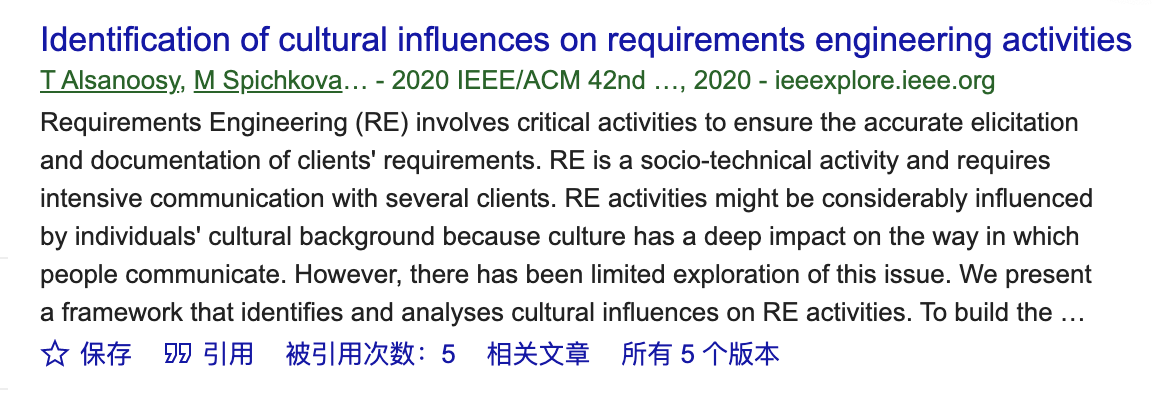
\includegraphics[width=0.3\textwidth]{./img/iden.png}\\
    \caption{\label{fig:iden1}Paper Citations}
\end{figure}

This article\cite{alsanoosy2020identification} is authored by Tawfeeq alsanoosy and submitted to icse 2020. It mainly discusses that since the user groups that software developers may face are from different regions or countries with different cultural backgrounds and different communication habits, the actions of software engineers to efficiently explore user needs have brought great challenges. This paper analyzes this phenomenon and gives its own solution.
The author first conducts modeling in the article. 
He uses Hofstede's definition and model of national cultural background (the most comprehensive system in cross-cultural research at present). In Hofstede's model, culture can be quantified by six dimensions, They are power distance index (PDI), individualism/collectivism (IDV), Masculinity/frmininity (MAS), Long-/Short-Term Orientation (LTO), Indulgence/impulses (IDN), Uncertainty Avoidance Index (UAI). Instead of using all six dimensions, the impact of culture on demand analysis is divided into sixteen aspects, which are respectively mapped to the four dimensions of PDI, IDV, UAI, and LTO among the above six dimensions (there are two more Dimensions have little impact on demand analysis), the following is the weight table established by the author.

\begin{table}[h]
\centering
\caption{\label{tab:widgets}IDV cultural influences on RE activities.}
\end{table}
\begin{figure}[h]
    \centering
    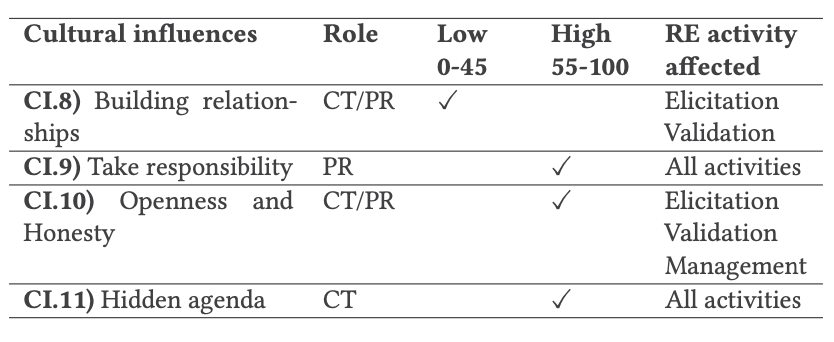
\includegraphics[width=0.3\textwidth]{./img/identable.png}\\
\end{figure}
With the above mapping table in hand, the authors use the following framework to analyze specific groups and finally generate a set of strategies to mitigate the impact of different cultural backgrounds on needs analysis. At the end of the paper, it is mentioned that the above-mentioned framework has achieved 89\% of the impact of Thai culture on demand analysis, and 75\% of Chinese culture, which shows that its effect is not bad.

\subsubsection{Why is this paper interesting?}

This paper analyzes the possible effects of different cultural backgrounds on demand mining and analysis, and proposes a plan that can effectively reduce the above effects in the cultural backgrounds of my country and Thailand. In the software requirements engineering class, the open source project analysis platform we want to develop is also like facing users of different cultures, facing different open source platforms, such as github, gitee, codeforge, etc., we also need to consider users of different platforms From this perspective, the issues discussed in this paper are highly related to the project we are going to do.

\subsection{RM2PT: A Tool for Automated Prototype Generation from Requirements Model}
\ \\
\begin{figure}[h]
    \centering
    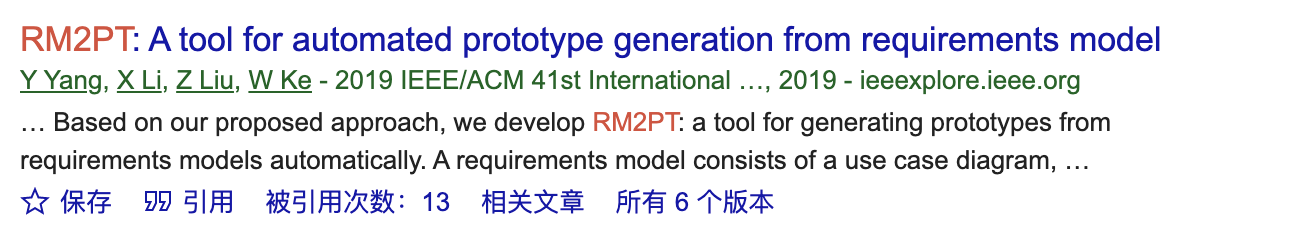
\includegraphics[width=0.3\textwidth]{./img/rm2pt.png}\\
    \caption{\label{fig:iden2}Paper Citations}
\end{figure}

\subsubsection{Introduction to the paper} 
The author of this article\cite{yang2019rm2pt} is Yang Yilong, an assistant professor at Beihang University, and submitted to icse 2019. It mainly discusses how to quickly visualize user requirements and generate prototypes in the face of abstract, vague and uncertain user requirements.
Specifically, the author uses java to implement a rapid prototype generator, which can quickly visualize demand models, including use case diagrams, concept class diagrams, etc., establish a list of contacts between different objects in a short time, and can communicate with The system sequence diagram is compared to check whether the pre-conditions, post-conditions and invariants input by the system are always established during the running of the program, and samples can also be input for system testing, which greatly shortens the software development engineer's analysis and analysis of requirements. Understanding time accelerates software development iterations. Users and other stackholders can also check whether their requirements are truly understood and satisfied by programmers by observing the generated use cases and requirement models, so as to avoid requirements analysis errors and project development failures.

\begin{figure}[h]
    \centering
    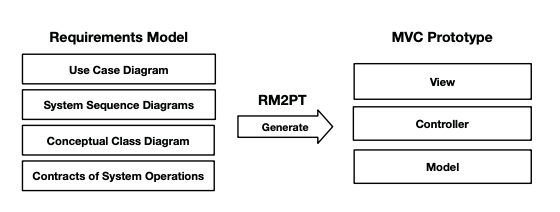
\includegraphics[width=0.3\textwidth]{./img/rm2pt_fig1.png}\\
    \caption{\label{fig:iden3}MVC Prototype Generation from Requirements Model }
\end{figure}

\subsubsection{Why is this paper interesting?}
The interesting thing about this article is that it mentions that the input to the rm2pt software is not only the requirement model mentioned above, but also the UML file, which is one of the topics we will learn in this course. I will try this software while learning UML, maybe it can help me understand the needs of users.

\subsection{Uncertainty-wise Requirements Prioritization with Search}

\begin{figure}[h]
    \centering
    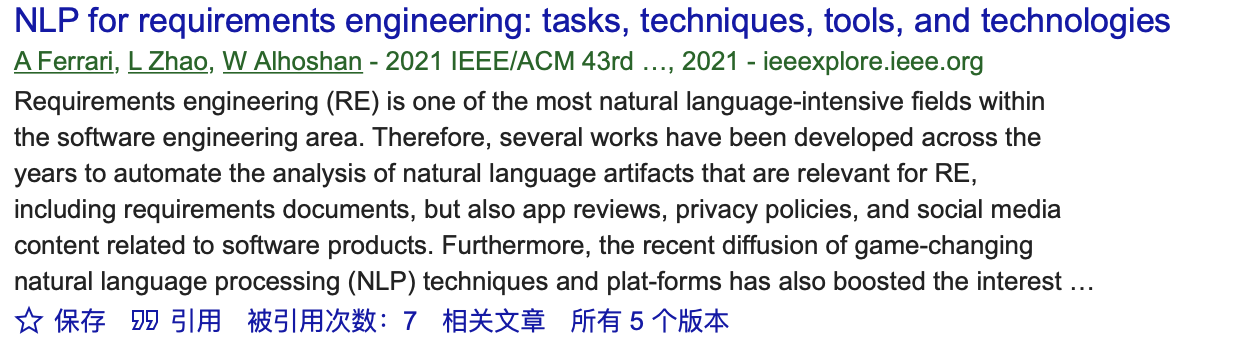
\includegraphics[width=0.3\textwidth]{./img/nlp_cite.png}\\
    \caption{\label{fig:iden4}Paper Citation }
\end{figure}

\subsubsection{Introduction to the paper}
This article\cite{zhang2020uncertainty} was submitted to TOSEM. It mainly discusses how to conduct scientific analysis and review in the face of the requirements of many users, prioritize these requirements, and reduce cost overruns by completing these requirements one by one according to the priority. Possibilities and uncertainties to ensure smooth software development. In the paper, the author proposes that the development priority of requirements should be determined according to the importance of requirements, the dependencies of requirements, the realization cost of requirements and the probability of cost overruns of requirements. In this paper, the author discusses the method, process and effectiveness of using NSGA, MO Cell, SPEA2 and other algorithms for demand priority calculation, and finally looks forward to the broad application fields of the algorithm in the future, which is relatively forward-looking.
\subsubsection{Why is this paper interesting?}
In daily development, we will encounter such a situation: there are many requirements to be implemented, but our time is limited, and the tasks to be completed must be sorted to ensure that we solve the most urgent and important requirements first, and this article The article gave us how to solve such a need and opened up my horizons.
\bibliographystyle{alpha}
\bibliography{citation}

\end{document}